% !TeX spellcheck = en_US
\documentclass[a4paper, 11pt]{article}
\usepackage[utf8]{inputenc}
\usepackage{t1enc}
\usepackage[english]{babel}
\usepackage{lmodern}
\usepackage{url}
\usepackage{graphics}
\usepackage{listings}
\usepackage{amssymb}
\usepackage{pifont}
\usepackage[a4paper, total={5.5in, 8in}]{geometry}

\hyphenation{UPPAAL}
\sloppy

\begin{document}
	
	\newcommand{\cmark}{\ding{51}}%
	\newcommand{\xmark}{\ding{55}}%
	
	\newcommand{\specialcell}[2][c]{%
		\begin{tabular}[#1]{@{}c@{}}#2\end{tabular}}
	
	\newenvironment*{mytable}[3]{
		% #1: caption, #2: cimke, #3: oszlopdef		 
		\begin{table}[htbp]	
			\caption{#1}          
			\label{tab:#2}            
			\center%
			\begin{tabular}{#3}
			}
			{
			\end{tabular}
		\end{table}
	}
	
	\pagestyle{plain}
	
	
	
	% angol környezet beállítása
	\nonfrenchspacing
	\setlength{\parindent}{0em}
	\setlength{\parskip}{0.45em}
	
	\title{A Cyber-Physical System:\\Controlling the CO$_2$ Concentration of the Air in a Greenhouse}
	\date{}
	\author{Bence Graics}	
	
	\maketitle
	\tableofcontents
	\newpage
	\section*{Introduction}
	This document introduces the implementation of a cyber-physical system (CPS) prototype, whose task is to keep the \emph{carbon-dioxide} concentration level of the air in a particular \emph{greenhouse} under an acceptable limit value.
	The greenhouse is an object with the approximate volume of a cubic meter. It has two \emph{windows} and a single \emph{fan}, which can be used to circulate the air in the object. The local elements of the presented CPS, which are located in the greenhouse, are the followings:
	\begin{itemize}
		\item a \textbf{CO$_2$ sensor}, capable of measuring the CO$_2$ concentration level of the air in the particular greenhouse,
		\item a \textbf{window handling engine}, capable of opening and closing the windows of the particular greenhouse,
		\item a \textbf{fan controller}, capable of turning the fan, located in the particular greenhouse, on and off.
	\end{itemize}
	
	In addition to controlling the CO$_2$ concentration level, the CPS has to provide additional services, called cloud services, that are located in the \emph{cloud}. The cloud services of the CPS are as follows. 
	\begin{itemize}
		\item \textbf{Historical data storage:} the CPS provides access to historical data with respect to the CO$_2$ concentration level of the air in the particular greenhouse.
		\item \textbf{Data visualization:} the CPS provides means to visualize historical data of the CO$_2$ concentration level of the air in the particular greenhouse.
		\item \textbf{Alert service:} the CPS send alerts when the CO$_2$ concentration level exceeds a certain limit value.
		\item \textbf{Timetable service:} the limit value of the CO$_2$ concentration can be different depending on whether there is human activity in the particular greenhouse or not. In the absence of human activity the limit value is higher in order to spare energy. The dates of human activity can be appointed using the timetable service, which are used by the CPS when calculating limit values.
	\end{itemize}
	
	The rest of the document presents the development process of the CPS. First, the most important high-level requirements regarding the CPS are introduced. Next, design and implementation details are presented for both the local components and the cloud services. Finally, thoughts and concluding remarks are shared.	
	
	\section{Requirements}
	\label{sec:requirements}
	This section presents the requirements the developed CPS has to meet. These requirements have been collected with the help of the owners of the greenhouse regarding the capabilities of the sensor and actuators. These requirements serve as the basis of the design upon which the implementation of the CPS is carried out (see Section \ref{sec:design}). The requirements are classified in accordance with the following aspects: functional requirements, extra-functional requirements and implementation constraints. Functional requirements are refined and partitioned into additional subclasses.
	
	\subsection{Functional Requirements}
	
	\paragraph{Sensing Capabilities}
	REQ-SC-1: The system shall sense the carbon-dioxide concentration of the air using a gas sensor at defined intervals.
	
	\paragraph{Actuating Capabilities}
	REQ-AC-1: The system shall open the windows of the greenhouse when the carbon-dioxide concentration is above normal level and the window is closed.
	
	REQ-AC-2: The system shall close the windows of the greenhouse when the carbon-dioxide concentration is on normal level and the window is open.
	
	REQ-AC-3: The system shall turn on the fan of the greenhouse when the carbon-dioxide concentration is above normal level and the fan is turned off. 
	
	REQ-AC-4: The system shall turn off the fan of the greenhouse when the carbon-dioxide concentration is on normal level and the fan is turned on.
	
	\paragraph{Accessible Services}
	
	REQ-AS-1: The system shall store historical data of carbon-dioxide concentration of the air in the greenhouse.
	
	REQ-AS-2: The system shall send alerts when the carbon-dioxide concentration of the air in the greenhouse is above a limit value.
	
	REQ-AS-3: The system shall support the visualization of stored data.
	
	REQ-AS-4: The system shall support the registration of dates that represent human activity within the greenhouse.
	
	REQ-AS-4-1: The system shall specify a lower limit value on the acceptable carbon-dioxide concentration level in the time of human activity. In the absence of human activity, the limit value is higher.
	
	\subsection{Extra-Functional Requirements}
	REQ-EF-1: The cloud services of the system shall be able to handle \textsl{1 message / 30 seconds} message rate. 
	
	REQ-EF-2: The messages from the greenhouse to the cloud shall be transferred via a secure channel.
	
	\subsection{Implementation Constraints}
	REQ-IC-1: The local components directly controlling the greenhouse shall operate on the Java platform\footnote{https://www.java.com/}.
	
	REQ-IC-2: Separate local components shall communicate using the Distributed Data Service\footnote{http://www.omg.org/spec/DDS/1.4} (DDS).
	
	REQ-IC-3: The cloud services shall run in the Microsoft Azure Cloud\footnote{https://azure.microsoft.com/}.
	
	\section{Design}
	\label{sec:design}
	This section introduces the design	choices upon which the implementation of the CPS is carried out. First, the system-level architecture is presented, which is followed by some low level (component level) design details.
	
	Figure \ref{fig:architecture} depicts the architecture of the designed CPS. The system consists of three bigger blocks: the greenhouse, a gateway and the cloud. 
		
		\begin{figure}[h!]
			\center
			\resizebox{140mm}{!}{
				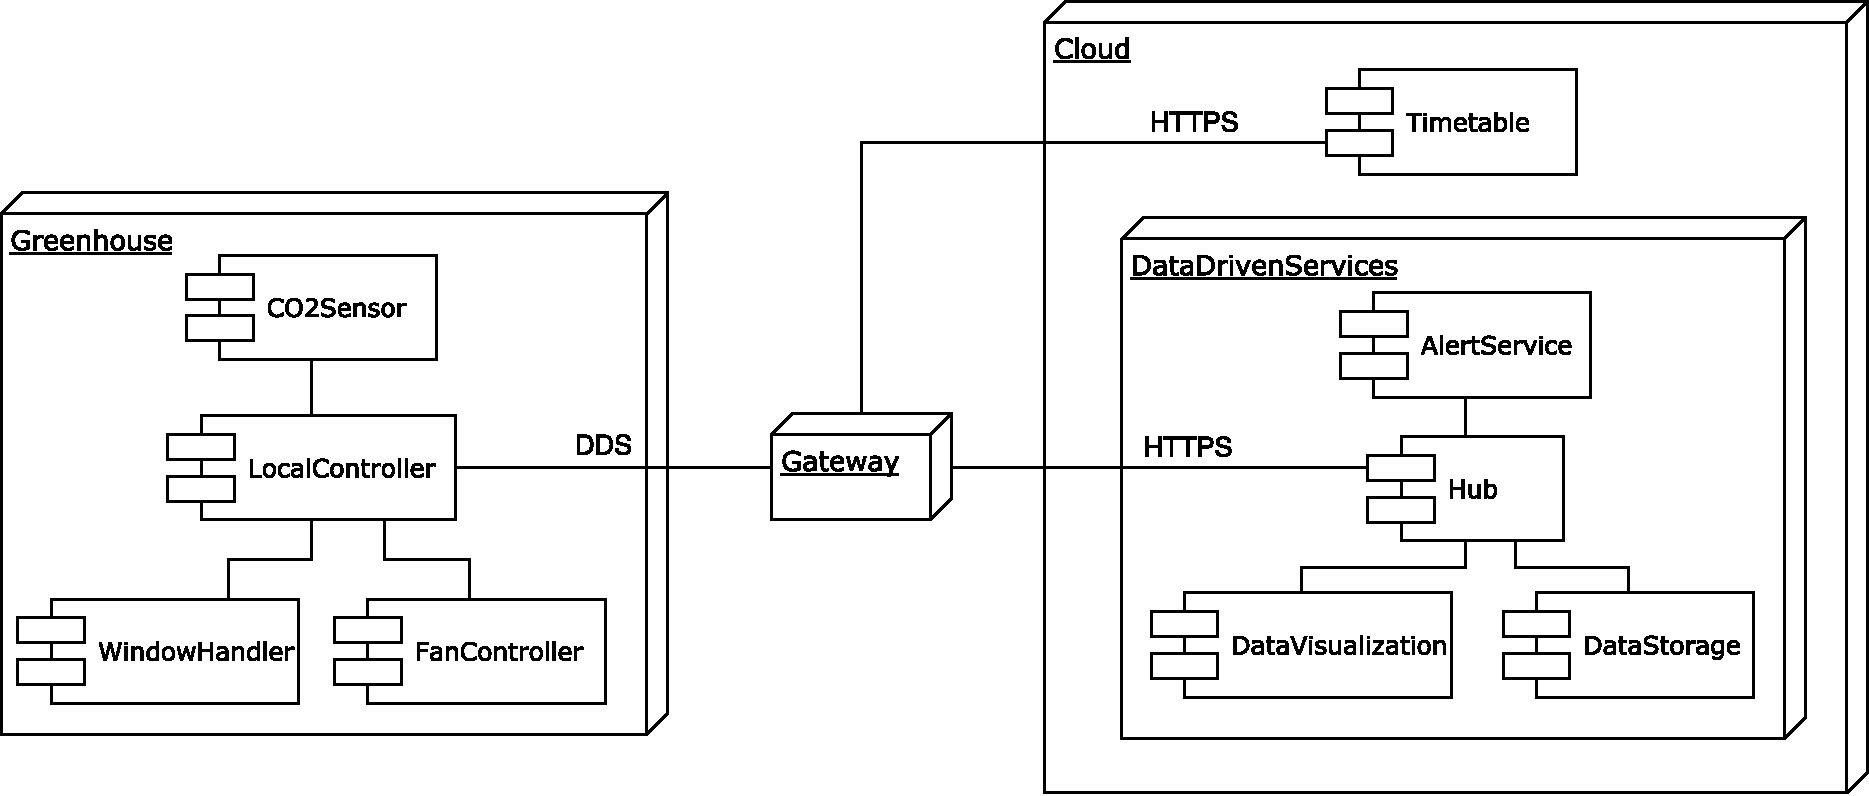
\includegraphics{fig/component-architecture.pdf}
			}
			\caption{The architecture of the CPS.}
			\label{fig:architecture}
		\end{figure}

	\subsection{Greenhouse}
	\label{sec:greenhouse}
	The \textbf{greenhouse}, as presented in the introduction, is the physical entity where the concentration of carbon-dioxide needs to be controlled. It has a single fan as well as two windows, which can be accessed using the \emph{fan controller} and the \emph{window handling engine} actuators. The CO$_2$ concentration level can be sensed using the \emph{carbon-dioxide sensor}. In this task we do not have to set or handle the greenhouse physically. Instead, the sensing and actuating activities can be accessed via well-defined DDS commands. The data structure of the commands is described by the following IDL\footnote{http://www.corba.org/omg\_idl.htm} code snippet.
	\begin{lstlisting}[
		basicstyle=\small, %or \small or \footnotesize etc.
	]
struct Greenhouse {
  string ID; //@key
  double Value;
  long TimeStamp;
};
	\end{lstlisting}
	
	Table \ref{tab:greenhouse-dds} summarizes the valid DDS commands that can be used for communication with the greenhouse on the DDS channel. Domain 0 is used for the communication. \emph{Topics} are used to segregate the command types.  Commands of certain topics can be \emph{read}, \emph{written} or \emph{read and written} by the greenhouse. The \emph{ID} of the command specifies the source (sensor) of particular data or concrete command (for actuation). The values of the commands specify particular data values (CO$_2$ concentration) or parameters of a certain command.
	
	\begin{mytable}{DDS commands of the greenhouse.}{greenhouse-dds}{|cccc|}
		\hline
		\textbf{Topic} & \textbf{ID} & \textbf{Read/Written} & \textbf{Values} \\ \hline \hline
		co2 & co2 & \xmark/\cmark & \specialcell{The CO$_2$ concentration of the air in \\ppm sensed by the built-in CO$_2$ sensor \\ of the greenhouse.} \\ \hline
		window & getwindow1 & \cmark/\xmark & \specialcell{The value field does not matter, \\ the greenhouse will return the state\\ of window1 in a command with id \textsl{window1}.} \\ \hline
		window & getwindow2 & \cmark/\xmark & \specialcell{The value field does not matter, \\ the greenhouse will return the state\\ of window2 in a command with id \textsl{window2}.}  \\ \hline
		window & window1 & \xmark/\cmark &  \specialcell{0 -- \textsl{window1} is closed, \\ 1 -- \textsl{window1} is open.} \\ \hline
		window & window2 & \xmark/\cmark &  \specialcell{0 -- \textsl{window2} is closed, \\ 1 -- \textsl{window2} is open.}  \\ \hline
		window & setwindow1 & \cmark/\xmark &  \specialcell{0 -- the greenhouse will close \textsl{window1}, \\ 1 -- the greenhouse will open \textsl{window1}.} \\ \hline
		window & setwindow2 & \cmark/\xmark &  \specialcell{0 -- the greenhouse will close \textsl{window2}, \\ 1 -- the greenhouse will open \textsl{window2}.} \\ \hline
		window & setvent & \cmark/\xmark &  \specialcell{0 -- the greenhouse will turn off the fan, \\ 1 -- the greenhouse will turn on the fan.} \\ \hline		
	\end{mytable}
	
	\subsection{Gateway}
	
	The task of the \textbf{gateway} is to control the carbon-dioxide level of the greenhouse using sensor data and utilizing its actuators. The communication between the greenhouse and the gateway is based on DDS, as presented in Section \ref{sec:greenhouse}. Furthermore, the gateway utilizes cloud services -- via the HTTPS protocol -- to ensure the quality of the controlling service and provide additional business services as defined in the requirements in Section \ref{sec:requirements}.	
	
	The operation of the gateway is simple, it is depicted in Figure \ref{fig:activity} using an activity diagram.
	
	\begin{figure}[h!]
		\center
		\resizebox{145mm}{!}{
			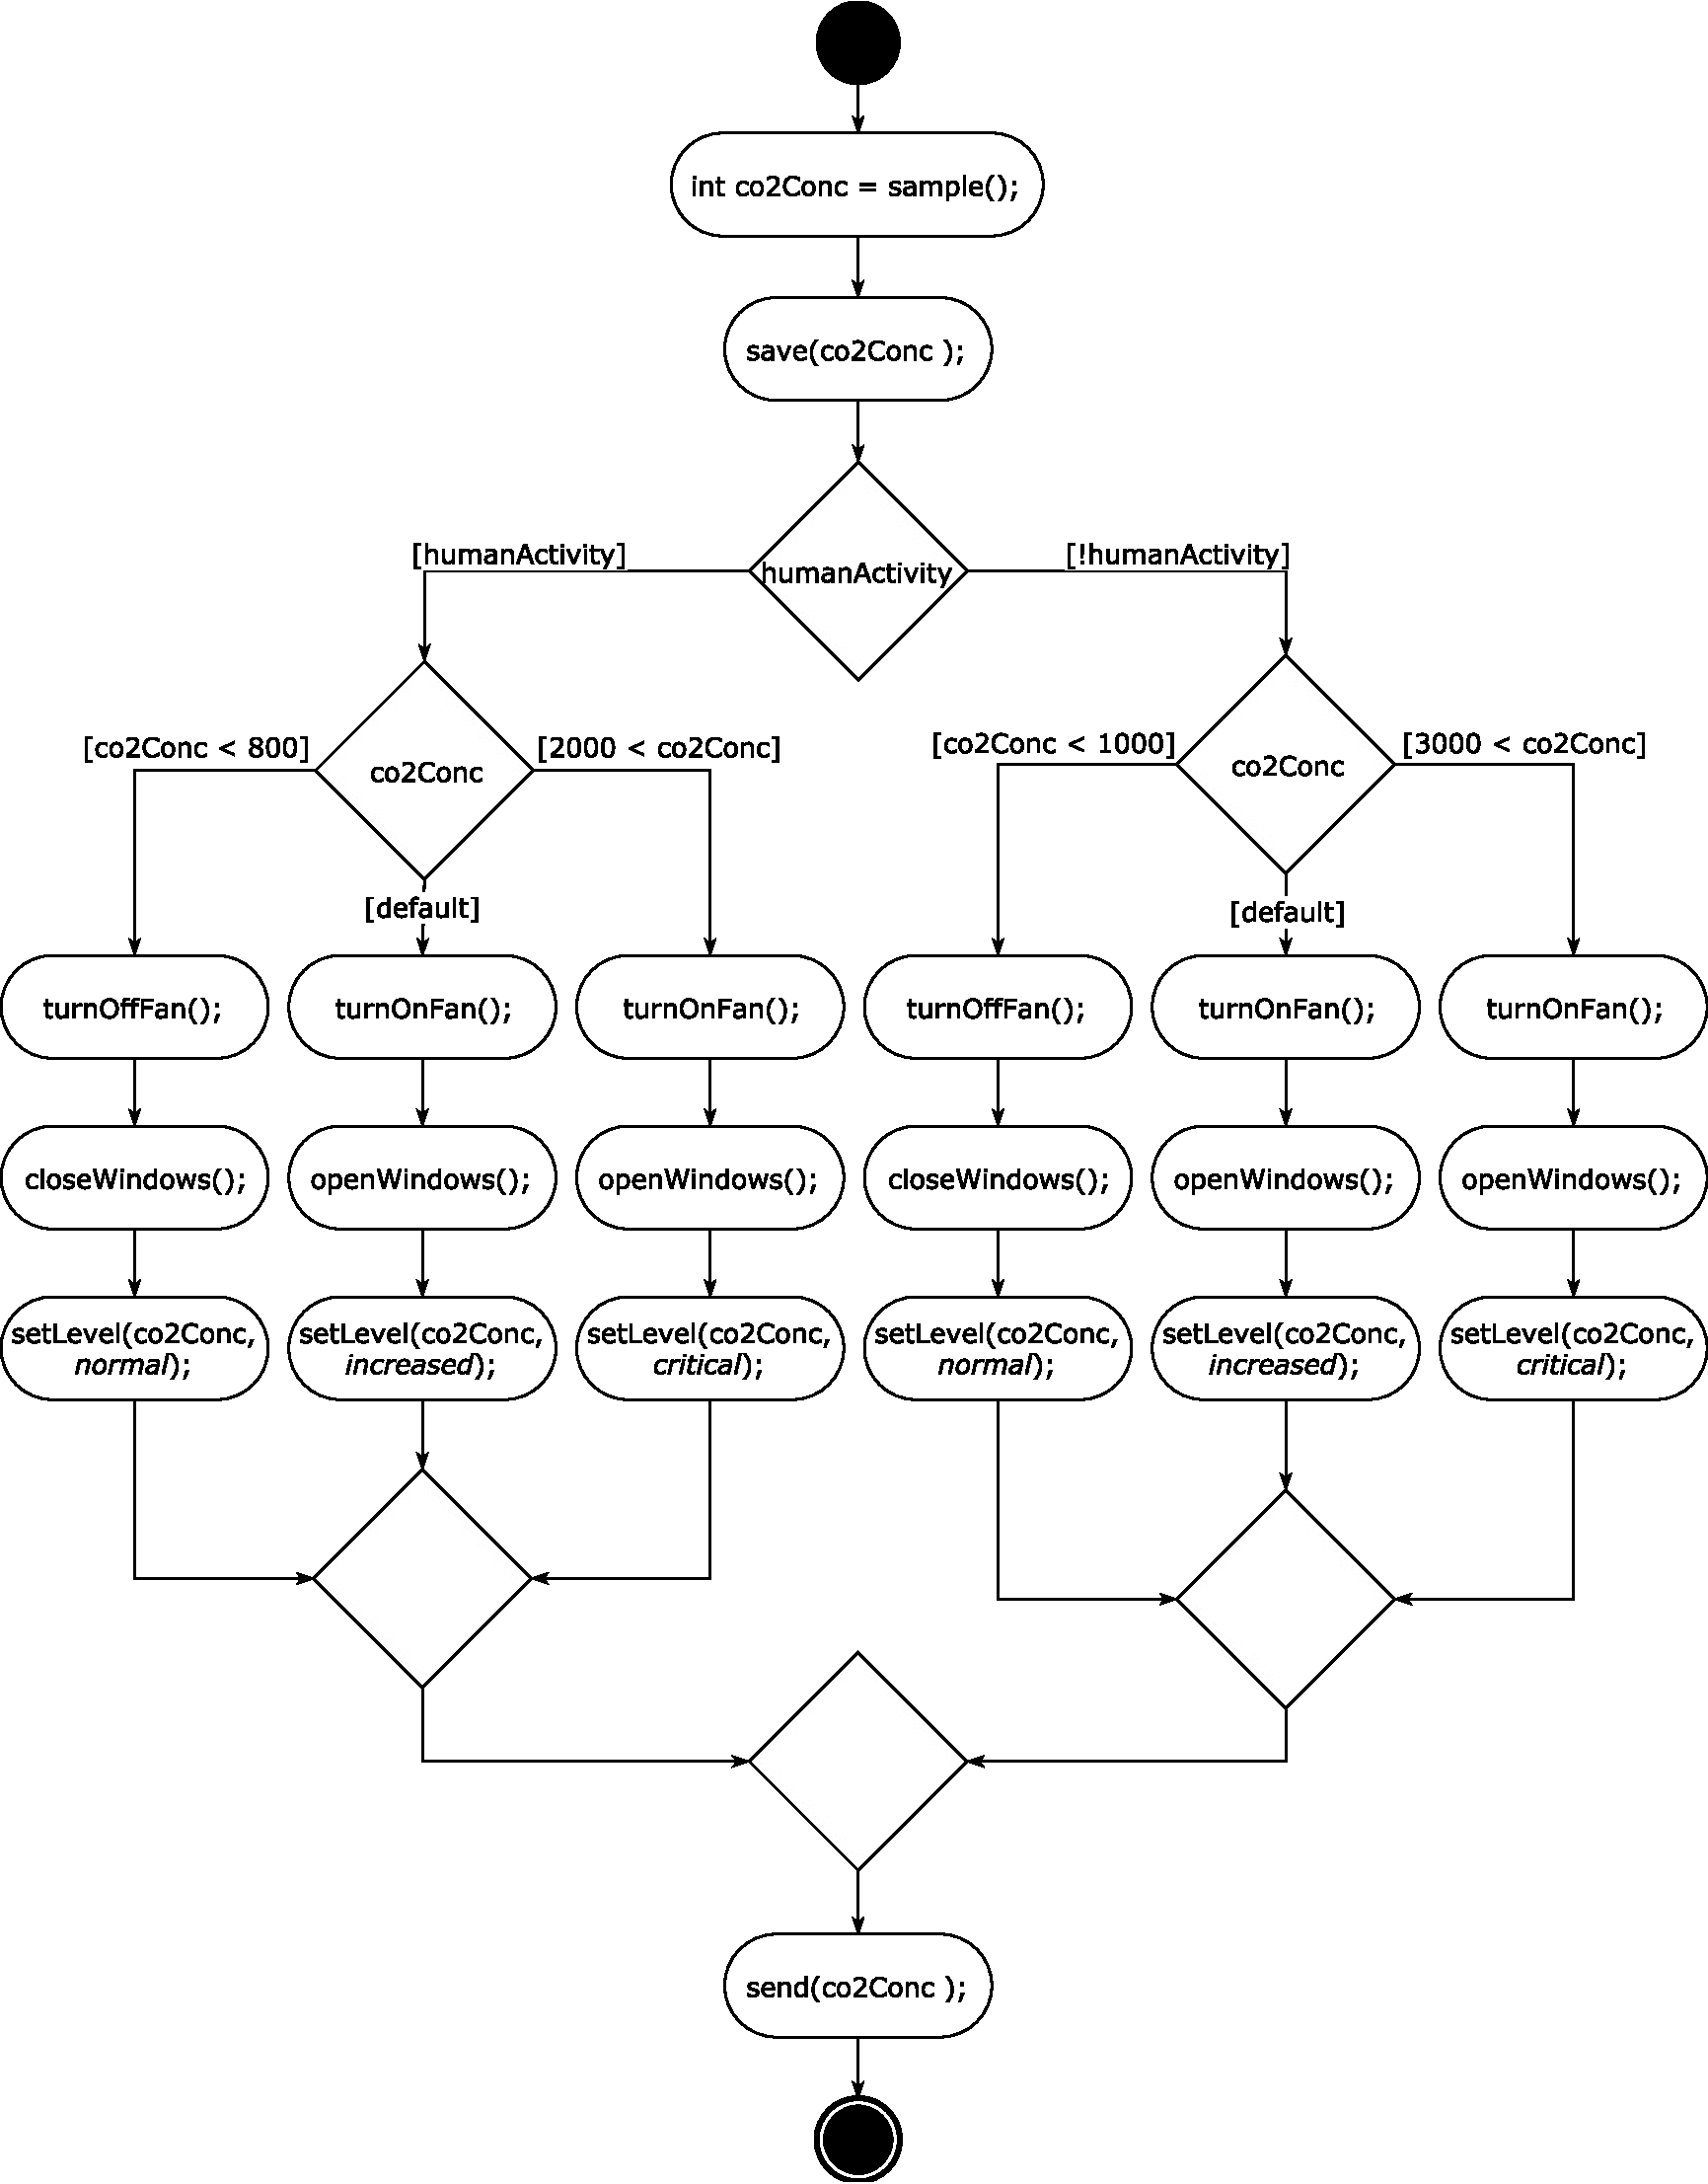
\includegraphics{fig/activity.pdf}
		}
		\caption{The activity diagram describing the periodic activity of the gateway.}
		\label{fig:activity}
	\end{figure}
	
	The gateway periodically samples the CO$_2$ concentration level of the air of the greenhouse. After sampling, it saves the value locally, thus a certain number of samples are available even if the cloud service is unreachable for a short period of time. 
	
	Further actions are based on the received concentration value as well as the data received from the timetable service. The logic reacts differently based on whether there is registered human activity in the room in the particular moment or not. To get this information, the gateway communicates with the timetable service periodically (e.g, every minute) and stores the answer. The limit values regarding the CO$_2$ concentration value with respect to human activity are specified by Table \ref{tab:limit-values}.
	
	\begin{mytable}{Limit values of CO$_2$ concentration in ppm with respect to registered human activity.}{limit-values}{|cccc|}
		\hline
		 & \textbf{Normal} & \textbf{Increased} & \textbf{Critical} \\ \hline \hline
		\textbf{Human activity} & Under 800 & Between 800 and 2000 & Above 2000 \\ \hline
		\textbf{No human activity} & Under 1000 & Between 1000 and 3000 & Above 3000 \\ \hline
		
	\end{mytable}
	
	If the CO$_2$ concentration of the air is on \emph{normal} level (regarding human activity in the room), the gateway sets the \textsl{level} attribute of the message that is to be sent to the cloud to \emph{normal}. Moreover, the gateway ensures that the windows are closed and the fan is turned off by sending the corresponding DDS commands to the greenhouse.  If the concentration level is \emph{increased}, the gateway sets the \textsl{level} attribute to \emph{increased} in addition to opening the windows and turning on the fans of the greenhouse. Finally, if the CO$_2$ concentration level is \emph{critical}, it sets the level attribute to \emph{critical}, in addition to initiating the necessary actuating activities. Finally, the gateway sends the message to the cloud in accordance with the following JSON format.
	
	\begin{lstlisting}[
	basicstyle=\small, %or \small or \footnotesize etc.
	]
{"id":"Id","value":951.39,"timeStamp":935971181,"level":"normal"}
	\end{lstlisting}
	
	\textsl{Id} serves as an identifier for the message, \textsl{value} indicates the CO$_2$ concentration of the air in the greenhouse. \textsl{TimeStamp} specifies the time of sending the message, and \textsl{level} indicates the level of the CO$_2$ concentration of the air. 
		
	As can be seen, the greenhouse with the gateway is responsible for implementing all \textsl{sensing} and \textsl{actuating} functional requirements: REQ-SC-1, and REQ-AC-1, REQ-AC-2, REQ-AC-3, REQ-AC-4. Furthermore, it partly implements accessible requirements REQ-AS-1 and REQ-AS-4-1. The messages are sent to the cloud via a secure channel to implement REQ-EF-2. Also, the logic is implemented in Java to meet REQ-IC-1. Finally, the communication with the greenhouse is based on DDS, thus, REQ-IC-2 is met.
	
	\subsection{Cloud Services}
	The \textbf{cloud} is used to provide special services regarding the control of th CO$_2$ concentration of the air in the greenhouse. All data sent to the cloud is stored on persistent containers. Also, the visualization of stored data is supported. Furthermore, depending on the \textsl{level} attribute of incoming messages, alerts (in the form of e-mails) can be sent to registered addresses. Finally, the timetable service holds information about human activity in the greenhouse.
	
	The cloud services -- apart from the timetable service -- are tightly integrated with each other. The timetable service is our custom implementation, whereas the other cloud services, to meet REQ-IC-3, are provided by Microsoft Azure Cloud.
	
	\subsubsection{Timetable Service}
	The timetable service is a custom implemented service reachable via a REST\footnote{https://en.wikipedia.org/wiki/Representational\_state\_transfer} API deployed on \emph{local host} on port 8080. To reach the service a GET message has to be sent to the following URL: \textsl{http://localhost:8080/hu.bme.mit.cps.timetable/timetable/timetable/activity}. The response is a JSON message in accordance with the following format.

	\begin{lstlisting}[
basicstyle=\small, %or \small or \footnotesize etc.
]
{"activity": false, "date": 1514581029369}
	\end{lstlisting}

	The \textsl{activity} attribute indicates whether there is human activity in the greenhouse when the server receives the request. The \textsl{date} attribute specifies the date of receiving the request of the client.

	The server maintains a very simple text file, which stores the dates of human activity in the greenhouse. The text file contains entries that conform to the following format:
	\begin{lstlisting}[
basicstyle=\small, %or \small or \footnotesize etc.
]
{"entries": [
  {"activityName":"CPS lesson",
  "beginning":"Dec 8, 2018 1:15:00 PM",
  "end":"Dec 8, 2018 1:45:00 PM"}
]}
\end{lstlisting}
	The \textsl{activityName} attribute describes the activity taking place from the date described by attribute \textsl{beginning} to \textsl{end}.

	When the server receives a request, it checks whether there is an activity registered in the file whose \textsl{beginning} and \textsl{end} attributes include the the reception time of the request. If so, it returns a message with attribute \textsl{activity} set to \emph{true}, otherwise to \emph{false}.
	
	Due to this design, REQ-AS-4 is met.
	
	\subsubsection{Azure Services}
	
	Microsoft Azure provides a large variety of services, which can easily be tailored to our needs and requirements. The design of this CPS component consists of choosing the right Azure services and defining their integration. The chosen Azure services are as follows:
	\begin{itemize}
		\item IoT Hub for
	\end{itemize}
	Figure \ref{fig:azure-cloud} depicts the integration of the data and alert services of the CPS.
		
	\begin{figure}[h!]
		\center
		\resizebox{135mm}{!}{
			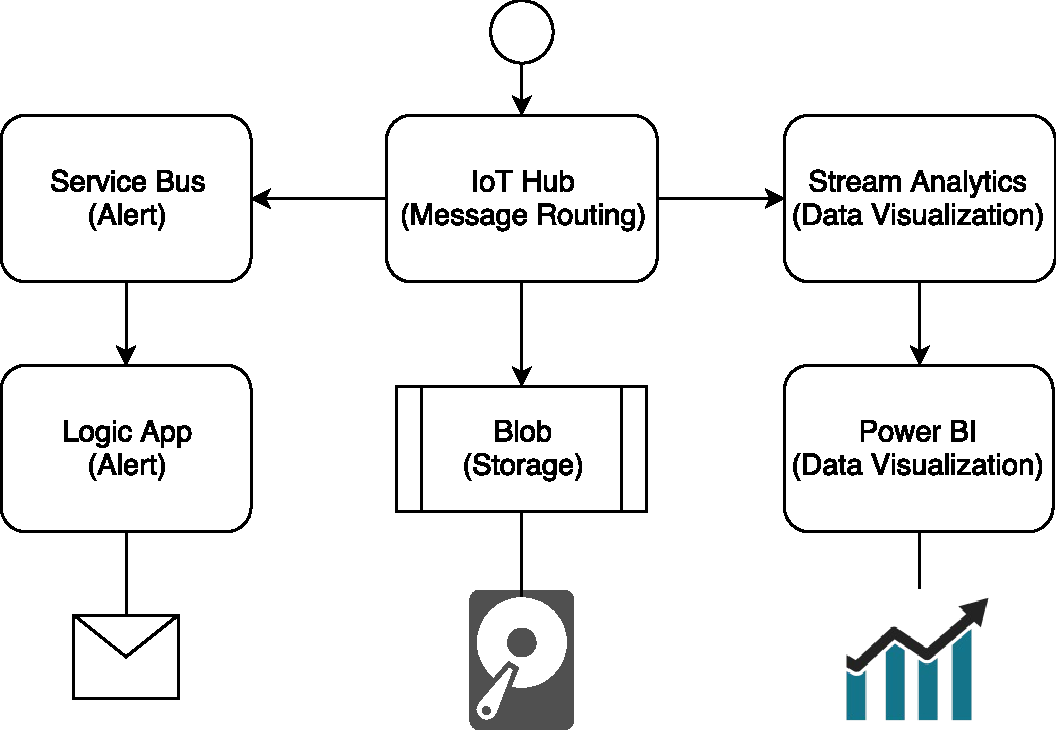
\includegraphics{fig/cloud.pdf}
		}
		\caption{The data flow in the cloud.}
		\label{fig:azure-cloud}
	\end{figure}
	
	Each message transmitted to the cloud is first processed by the IoT Hub. This is the central element in the cloud. It is 	capable of routing incoming messages to other service nodes based on certain properties. The additional services are as follows.
	 \begin{itemize}
	 	\item Each message is transferred to the blob and saved (persistent storage).
		\item Each message is transfered to the stream analytics service that sends the data to the visualization service.
	 	\item If the alert property of a message is \textsl{true}, then a message is transmitted to the alert service bus. The service bus stores the messages in its queue and forwards them one-by-one to the alert logical app. The logical app is responsible for sending e-mails to the specified addresses.
	 \end{itemize}
	
	\section{Implementation}
	\label{sec:implementation}
	This section presents the implementation details of the CPS based on the design introduced in Section \ref{sec:design}. The implementation details are partitioned into a local aspect, describing the details of the gateway implementation, and aspect of the cloud services. In both cases, the introduction starts with necessary technological environment, which is followed by a detailed guide on creating a functioning system.
	
	\subsection{Local Aspects}
	
	\subsection{Aspect of Cloud Services}
	
	\section{Conclusion}
	
%	Figure \ref{fig:architecture} depicts the architecture of the implemented CPS. As can be seen, the system consists of three bigger blocks: the greenhouse, a gateway and the cloud. 
%	
%	\begin{figure}[h!]
%		\center
%		\resizebox{140mm}{!}{
%			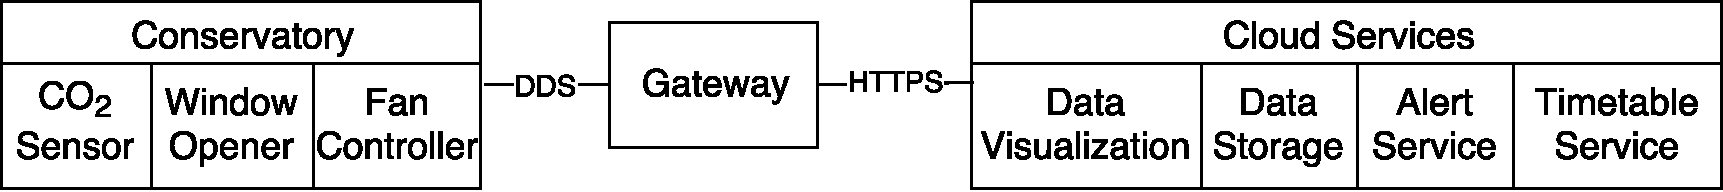
\includegraphics{fig/architecture.pdf}
%		}
%		\caption{The architecture of the CPS.}
%		\label{fig:architecture}
%	\end{figure}
%
%	The \textbf{greenhouse} is the physical entity where the concentration of carbon-dioxide needs to be controlled. It has a single fan, which can be used to circulate the air, as well as two windows, which can be opened and closed. Regarding sensors and actuators, the greenhouse contains a carbon-dioxide sensor in addition to the two window openers and a fan controller.
%	
%	The job of the \textbf{gateway} is to control the carbon-dioxide level of the greenhouse using its sensor and actuators. The communication between the greenhouse and the gateway is based on DDS. Furthermore, the gateway utilizes cloud services (via the HTTPS protocol) to ensure the quality of the controlling service.
%	
%	The \textbf{cloud services} (apart from the timetable service) are tightly integrated with each other. The data coming to the cloud is stored on persistent containers. Also, incoming data can be visualized. Furthermore, if certain values of the incoming data are too high, alerts can be sent. Finally, the timetable service holds information about the lessons taking place in the room represented by the greenhouse.
%	
%	\section{Gateway Functionalities}
%	This section introduces the most important functionalities of the gateway on a lower abstraction level. All gateway functionalities have been implemented in Java 8.
%	
%	After the gateway is initiated, it initializes the DDS infrastructure. It has a single reader entity, which reads the carbon-dioxide concentration on the particular topic where the gas sensor of the greenhouse publishes its data. Additionally, it has a writer entity responsible for publishing commands on the corresponding topic, which control the window opener and fan controller of the greenhouse in accordance with the sensed carbon-dioxide concentration level.
%	
%	The handling of incoming data is implemented in accordance with the activity diagram presented in the system design (see Figure \ref{fig:activity}).
%	
%	\begin{figure}[h!]
%		\center
%		\resizebox{140mm}{!}{
%			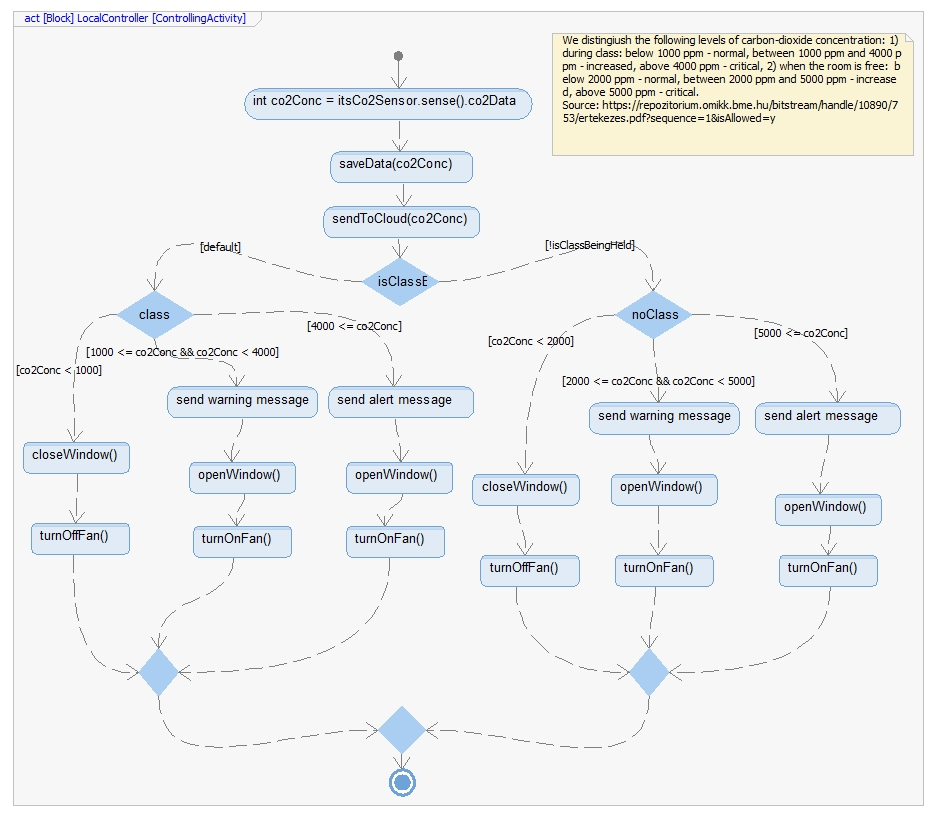
\includegraphics{fig/activity.jpg}
%		}
%		\caption{The activity diagram of LocalController.}
%		\label{fig:activity}
%	\end{figure}
%
%	The logic reacts differently based on whether there is a lesson taking place in the room in the particular moment or not. To get this information the gateway communicates with the timetable service periodically (every minute by default) and stores the answer. This communication takes place via a well-defined REST API:
%	\begin{itemize}
%		\item HTTP verb: GET.
%		\item URL where the request needs to be sent:		
%		http://152.66.181.77:8080/ \\ hu.bme.mit.cps.timetable/timetable/lesson.		
%		\item Answer: a JSON structure containing a \textsl{date} field with the date of the reply and a \textsl{lesson} field indicating whether there is a lesson held at the particular moment (true/false).
%		\begin{lstlisting}[
%		basicstyle=\small, %or \small or \footnotesize etc.
%		]
%{"date":"Dec 11, 2017 10:15:00 PM", "lesson":"true"}
%		\end{lstlisting}
%	\end{itemize}
%
%	Furthermore, the gateway communicates with the cloud each time it receives data from the greenhouse. This is achieved by using the \textsl{DeviceClient} class of the Azure Development Kit.
%	Each message transmitted to the cloud conforms to the following JSON format.
%	\begin{lstlisting}[
%		basicstyle=\small, %or \small or \footnotesize etc.
%	]
%{"id":"messageId","value":95.39,"timeStamp":925971383,
%"comment":"critical"}
%	\end{lstlisting}
%	
%	\section{Cloud Services}
%	This section introduces the cloud services on a lower abstraction level. The timetable has been implemented by the author, whereas the other services are based on the commercial services of Microsoft Azure\footnote{https://azure.microsoft.com/}.
%	
%	\subsection{Timetable Service}
%	The timetable service is based on the Maven WildFly 10.x server. On each request, it reads a local file that stores data about the reservations of the presented room. The data is stored in accordance with the following JSON structure:
%	\begin{lstlisting}[
%	basicstyle=\small, %or \small or \footnotesize etc.
%	]
%{"lessons":[
%{"lessonName":"CPS","beginning":"Dec 11, 2017 10:15:00 PM",
%"end":"Dec 11, 2017 11:45:00 PM"},
%{"lessonName":"SWSV","beginning":"Dec 11, 2017 12:15:00 PM",
%"end":"Dec 11, 2017 13:45:00 PM"}
%]}
%	\end{lstlisting}
%	As can be seen, the entries are stored in a list (\textsl{lessons}). An entry has the following fields: \textsl{lessonName} is a string value, whereas the \textsl{beginning} and \textsl{end} are two date value.
%	
%	The server logic is simple. When a request arrives, it checks whether there is an entry defining a lesson in the particular moment. Also, the server is responsible for deleting old entries to save storage space.
%	\subsection{Azure Services}
%	Figure \ref{fig:cloud} depicts the integration of the cloud services in Microsoft Azure.
%	
%	\begin{figure}[h!]
%		\center
%		\resizebox{125mm}{!}{
%			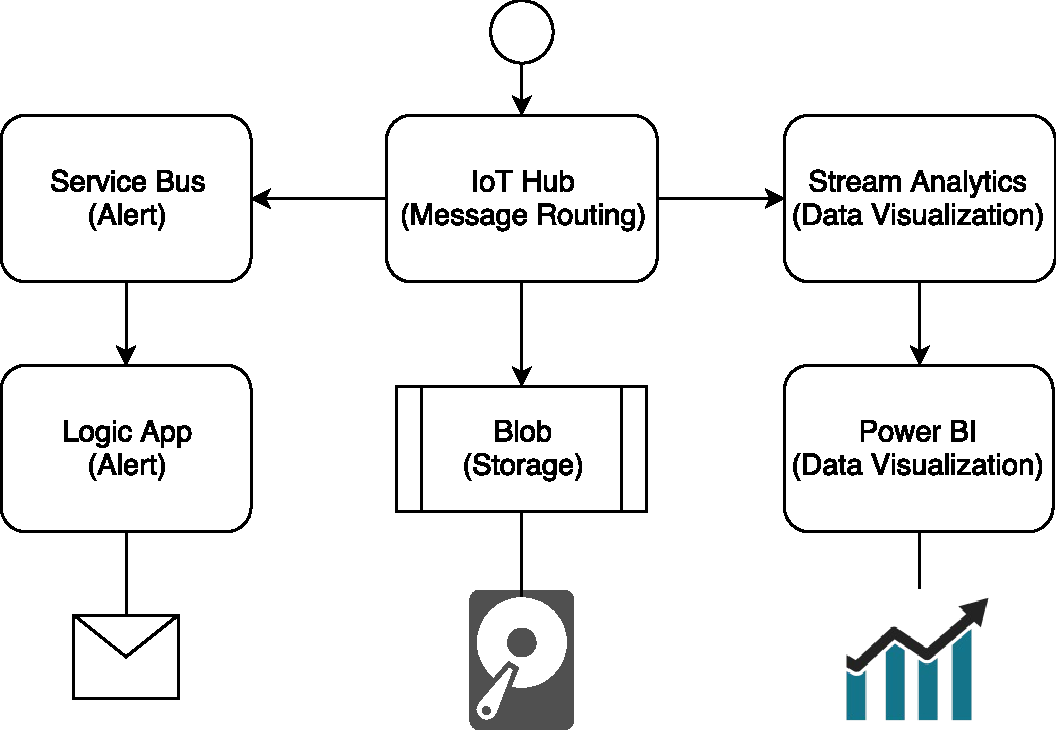
\includegraphics{fig/cloud.pdf}
%		}
%		\caption{The data flow in the cloud.}
%		\label{fig:cloud}
%	\end{figure}
%
%	 Each message transmitted to the cloud is first processed by the IoT Hub. This is the central element in the cloud. It is capable of routing incoming messages to other service nodes based on certain properties. The additional services are as follows.
%	 \begin{itemize}
%	 	\item Each message is transferred to the blob and saved (persistent storage).
%	 	\item Each message is transfered to the stream analytics service that sends the data to the Power BI visualization service.
%	 	\item If the alert property of a message is \textsl{true}, then a message is transmitted to the alert service bus. The service bus stores the messages in its queue and forwards them one-by-one to the alert logical app. The logical app is responsible for sending e-mails to the specified addresses.
%	 \end{itemize}	
	
\end{document}